\chapter{基于DMAIC的小微贷款服务质量根因分析与改进方案}

\section{DMAIC在本项目中的应用框架}

DMAIC方法论源自六西格玛管理体系，包含定义（Define）、测量（Measure）、分析（Analyze）、改进（Improve）和控制（Control）五个阶段，其核心逻辑是通过数据驱动的持续改进循环实现对业务流程质量的结构化提升\cite{ref12}。在金融服务领域，DMAIC已被应用于银行零售业务服务改善\cite{ref12}、银行网点服务管理优化\cite{ref51}以及金融科技客服运营延迟改进\cite{ref49}等场景，展现出对多触点、多环节服务流程的适配能力\cite{ref47}。\par

在本项目中，DMAIC并非作为僵化的五阶段模板机械套用，而是作为整合SERVQUAL服务质量测量的工程化管理闭环贯穿全文。五个阶段与论文章节的映射关系如下：Define阶段（第1至第3章）完成项目边界的定义——从普惠金融与小微贷款的宏观背景出发，收束至P公司服务质量现状的诊断与问题框架的建立；Measure阶段（第4章）构建改良SERVQUAL八维评价模型，通过486份有效问卷的期望-感知差距测量，获得P公司服务质量的量化基线；Analyze与Improve阶段（本章）承接第4章的测量数据，完成从关键短板归纳、根因追溯（5.2至5.3节）到五项工程化改进方案设计（5.4至5.8节）的全过程；Control阶段（第6章）负责实施保障、效果评价与持续控制机制的设计。整个闭环的逻辑起点是P公司业务痛点，逻辑终点是可持续的服务质量提升机制。DMAIC五阶段与论文章节映射如表\ref{tab:5-1}所示。\par

\begin{table}[htbp]
  \centering
  \small
  \caption{DMAIC五阶段与论文章节映射}
  \label{tab:5-1}
  \scalebox{0.85}{%
  \begin{tabular}{p{0.12\textwidth} p{0.20\textwidth} p{0.34\textwidth} p{0.34\textwidth}}
    \toprule
    \textbf{DMAIC阶段} & \textbf{论文章节} & \textbf{核心任务} & \textbf{关键产出} \\
    \midrule
    Define & 第1章至第3章 & 界定项目边界与服务质量问题 & P公司服务流程诊断、问题框架 \\
    Measure & 第4章 & 构建评价模型并测量服务质量差距 & SERVQUAL八维模型、期望-感知差距数据 \\
    Analyze & 第5章（5.2-5.3） & 归纳关键短板并进行根因分析 & 鱼骨图、5Why根因链 \\
    Improve & 第5章（5.4-5.8） & 设计工程化改进方案 & 五项可执行改进方案 \\
    Control & 第6章 & 实施保障、效果评价与持续控制 & WBS、RACI矩阵、控制看板 \\
    \bottomrule
  \end{tabular}%
  }
\end{table}

上述框架的核心优势在于：SERVQUAL测量提供了短板识别的量化依据，DMAIC提供了从诊断到改进再到控制的完整闭环路径，两者整合后使服务质量改进不再是零散的专项行动，而是具有工程化特征的系统管理过程。\par

\section{关键服务质量短板归纳}

基于第4章SERVQUAL八维期望-感知差距测量和IPA四象限分析结果，本文从P公司小微贷款服务质量数据中提炼出以下五个关键短板，作为后续根因分析和改进方案设计的基础。\par

短板一：信息透明度不足。透明性维度的期望-感知差距为-1.70，在八个维度中负向差距最大。其中退件原因明确性（SQ23）的满意度仅为2.80/5.0，审批进度实时查询（SQ22）的满意度为3.25/5.0，两者均落入IPA"高重要-低满意"象限。这表明客户对审批进度不可见、退件通知笼统（如仅告知"材料不齐全"而不指明具体缺失项）、费用结构事先不清晰等问题存在强烈的改进期待\cite{ref15}。信息透明度不足直接导致客户反复补正、信任度下降，进而推高材料补正率（28\%）和退件率（8\%）。\par

短板二：响应速度慢。响应性维度的期望-感知差距为-1.53，是负向差距第二大的维度。审批时效承诺（SQ01）的满意度仅为2.95/5.0，与客户的强期待（重要度4.52/5.0）形成尖锐落差。从实际运营数据看，授信审批的实际中位数耗时达12个工作日，远超出对外承诺的7个工作日，超时率达26\%。补正通知的延时加剧了客户焦虑，而客户经理电话接通率低（3次内接通率不理想）进一步放大了客户对响应迟缓的负面感知。\par

短板三：资料流程繁琐。便利性维度的期望-感知差距为-1.15，其中材料一次告知明确性（SQ18）的满意度为3.10/5.0，全流程线上可操作性（SQ17）的满意度为3.40/5.0，二者均处于IPA优先改进象限。P公司当前的材料补正率为28\%，意味着每3.6笔申请中就有1笔需补充材料，首轮一次通过率仅为62\%。反复补正不仅拉长了客户的等待时间（平均办理时长12个工作日，75分位数达20个工作日），也增加了客户经理的重复沟通工作量。\par

短板四：产品匹配度弱。产品适配维度的期望-感知差距为-1.23，贷款方案匹配度（SQ25）满意度仅为3.15/5.0，处于IPA优先改进象限的边界位置。P公司当前提供的小微贷款产品（信用贷、担保贷、供应链贷三类）虽覆盖了主要融资场景，但标准化产品方案难以匹配处于不同生命周期（初创期、成长期、成熟期）的客户在额度、期限和还款方式上的差异化需求。产品匹配不足直接影响客户的续贷意愿和转介意愿，是制约客户生命周期价值释放的关键因素。\par

短板五：投诉闭环管理薄弱。投诉闭环率仅为62\%，重复投诉率高达23\%。投诉处理时效承诺（SQ08）的满意度为3.55/5.0，虽未落入IPA优先改进象限，但结合运营数据看，62\%的闭环率意味着38\%的投诉在5个工作日内未得到实质性解决。更严重的问题是：现行投诉处理机制缺少根因回溯环节，同类问题反复发生——审批时效慢（占比32\%）和材料要求不清晰（占比22\%）两项合计占投诉总量的54\%，但数月至一年后仍未观察到系统性改善，这正是"重处理、轻分析、无回溯"的典型症状。\par

上述五个短板覆盖了客户旅程的核心触点——申请与资料准备、审批进度关注、产品方案选择、客户经理交互、以及投诉后的服务补救，形成了从"事前-事中-事后"的完整问题链。\par

\section{根因分析}

为深入揭示上述五个服务短板的深层成因，本文采用鱼骨图分析方法，从人员、流程、系统、产品、制度、风险六个维度进行结构化根因追溯，并结合5Why追问法逐层拆解至可干预的管理节点。服务质量短板鱼骨图如图\ref{fig:5-1}所示。\par

\begin{figure}[htbp]
  \centering
  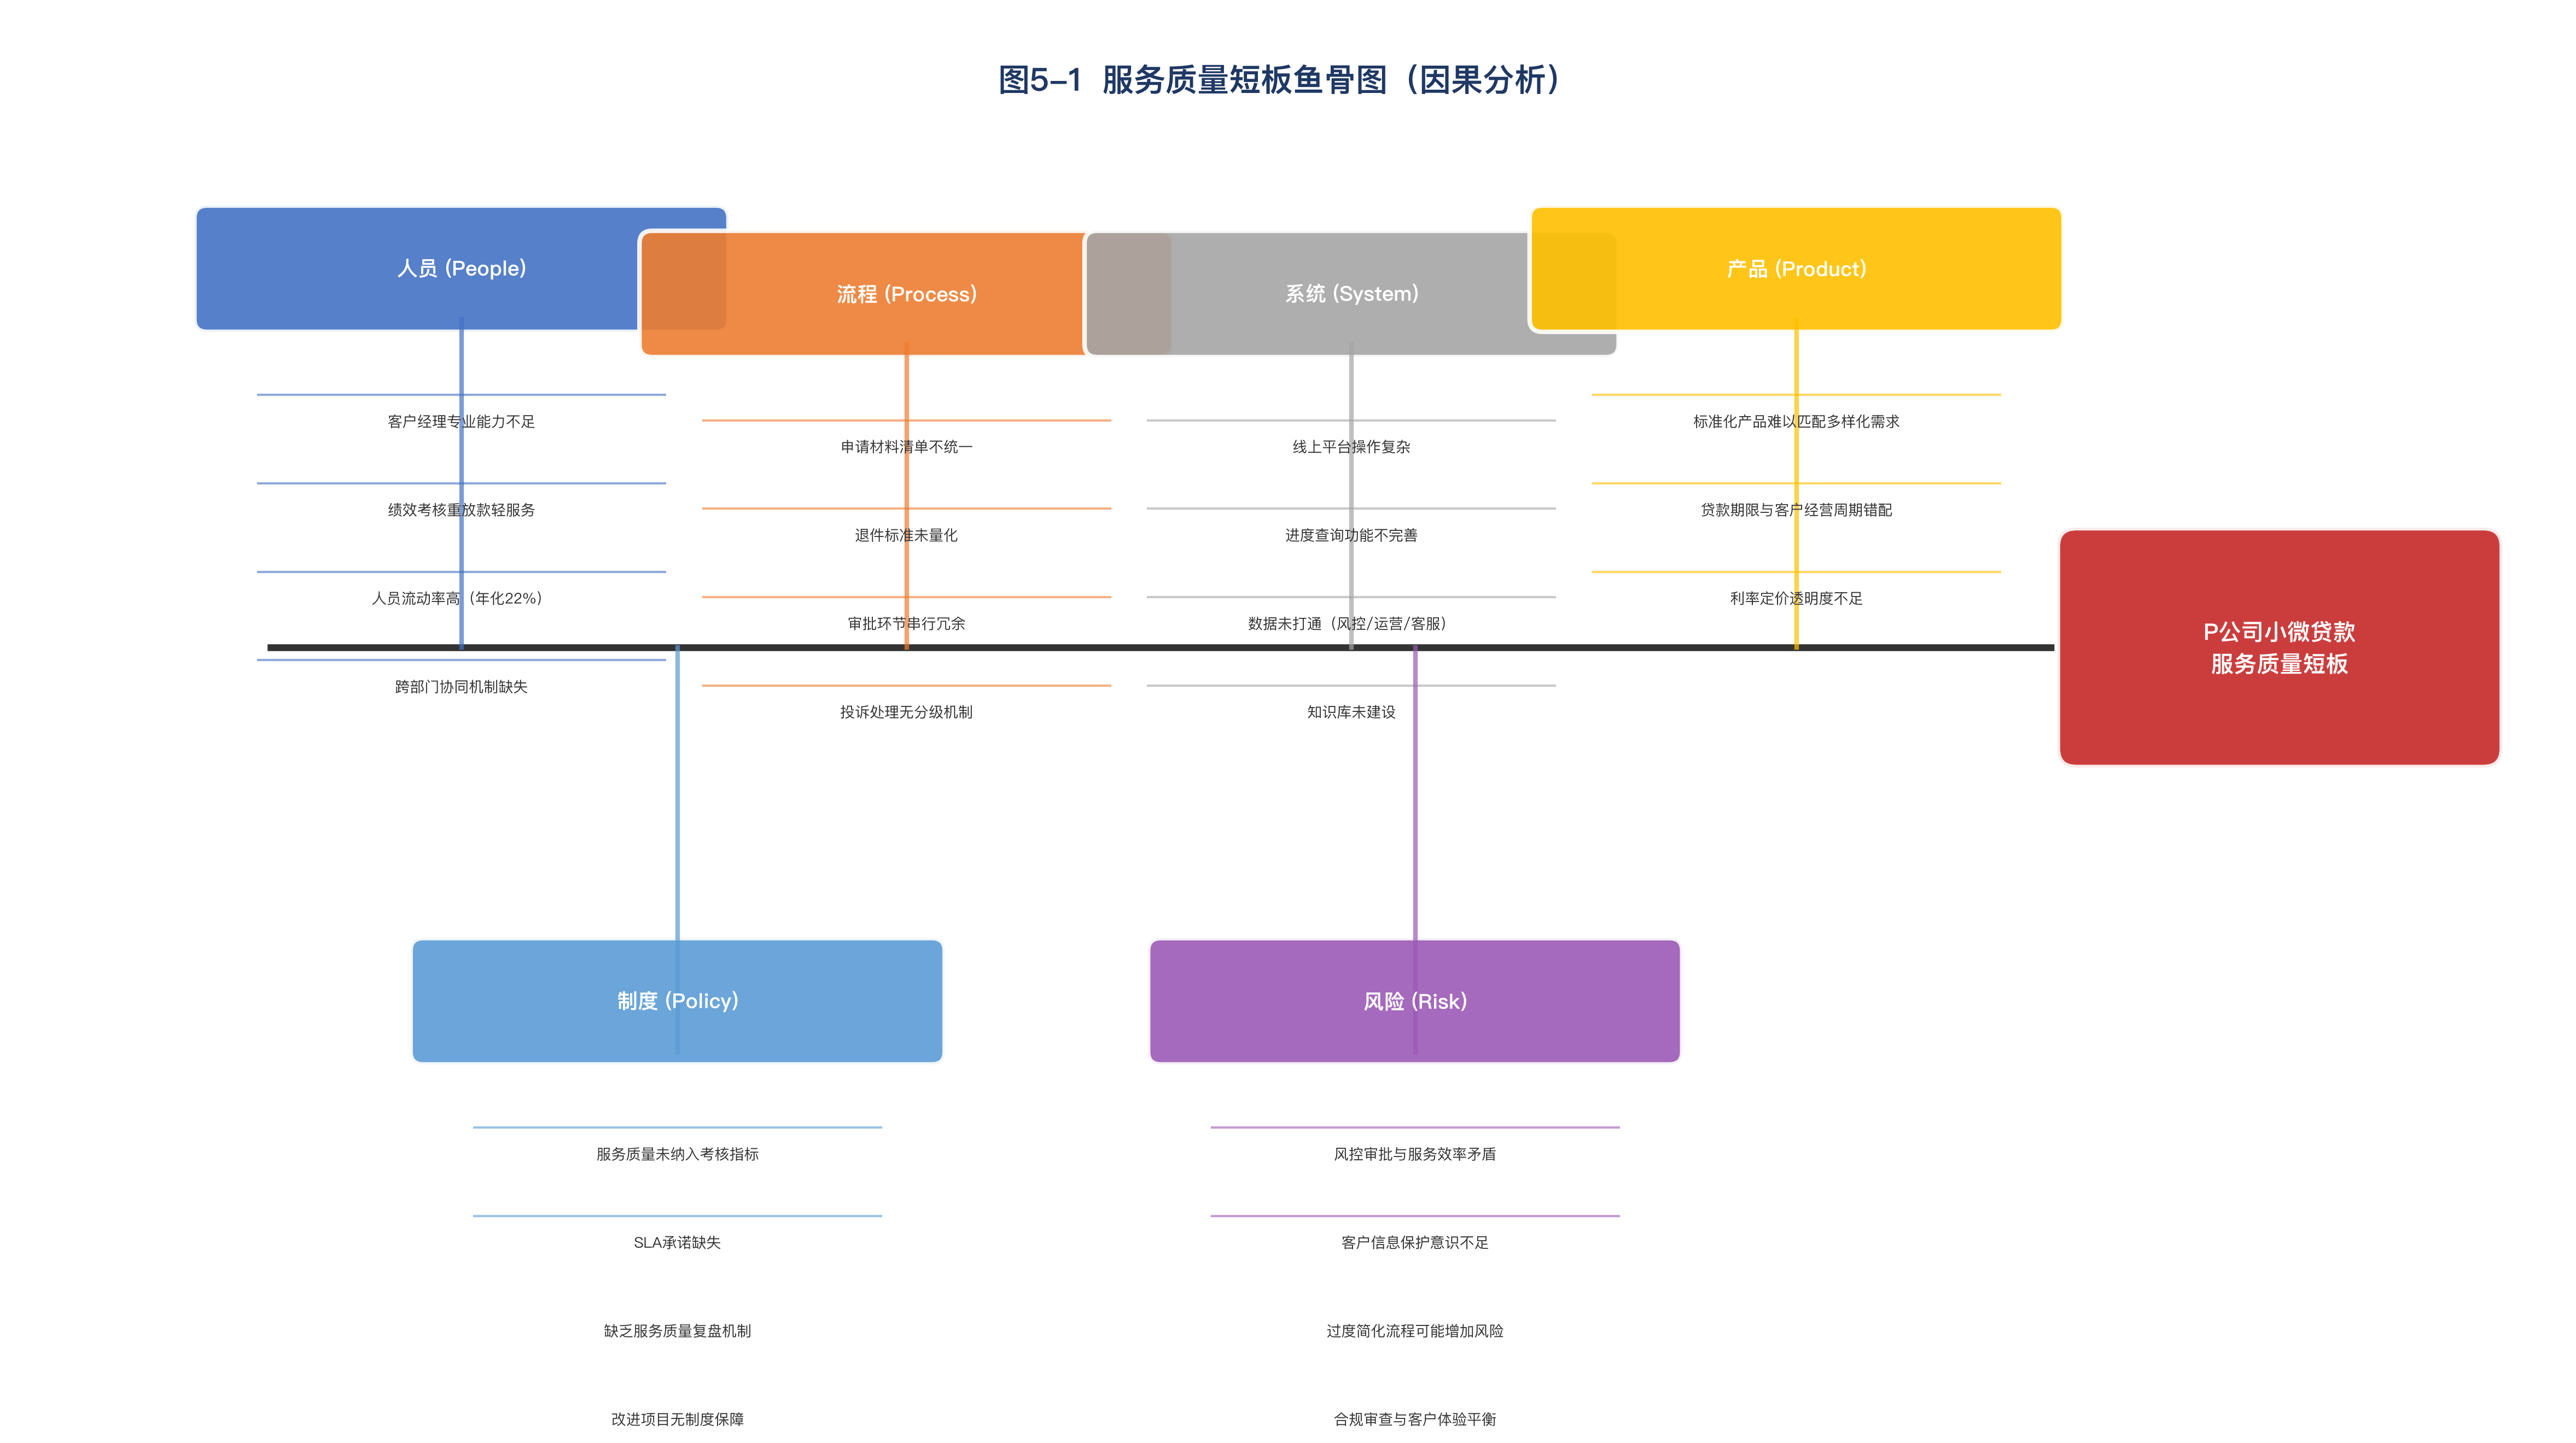
\includegraphics[width=0.85\textwidth]{figures/图5-1_服务质量短板鱼骨图.png}
  \caption{服务质量短板鱼骨图}
  \label{fig:5-1}
\end{figure}

\subsection{人员维度}

P公司客户经理团队约45人，其中入职不满2年的新客户经理占比约40\%。这些新客户经理在独立面对客户时，专业知识储备不足（Why：培训体系不健全，现行的入职培训以产品手册自学为主、非结构化师徒带教为辅，缺少标准化的产品知识体系培训课程），导致不同客户经理在回答贷款方案、利率政策、还款方式等同类问题时口径不一致，客户感知到的专业度大打折扣。进一步追问（Why：无标准化知识库），客户经理在提交申请材料时的审核判断依赖个人经验，而非统一的材料清单和判定标准，这使得同一客户面对不同客户经理时可能获得不同的材料要求说明，间接推高了补正率。更深层的原因是绩效考核导向的偏差：现行客户经理KPI仅考核放款量（Why：管理层未将服务质量纳入绩效设计），导致客户经理行为趋利化——追求个人放款量最大化，主动忽视服务的及时性和客户沟通质量。张磊等的研究表明，政策扶持与金融科技的协同效应是改善小微企业融资环境的关键路径，单一维度的改进（如仅增加信贷供给）难以产生实质性效果，这一判断为本研究从人员、流程、系统、产品、制度和风险六个维度同步发力的改进策略提供了方法论启示\cite{ref52}。\par

\subsection{流程维度}

P公司的资料补正环节是造成流程效率低下的关键瓶颈。客户在提交申请后收到的补正通知通常表述笼统（如"请补充相关财务资料"），缺少对具体缺失项和提交标准的明确说明（Why：无标准化补正模板，客户经理通过系统自由文本框输入补正要求），客户需要反复与客户经理电话确认才能使材料达标，导致退件率上升。投诉处理流程同样存在结构性缺陷：现行机制未建立投诉分级规则（Why：缺少客服SOP文件），所有投诉统一进入工单池，按时间先后顺序处理，而非按紧急程度和影响程度分级响应。黄玉婷在客户服务流程改进研究中强调，缺少分级机制是导致服务响应效率低下的系统性原因\cite{ref53}。低级别投诉因处理优先级靠后而被长期搁置，当同一客户问题未得到及时解决时，低级别投诉便升级为重复投诉乃至客户流失事件。\par

\subsection{系统维度}

P公司当前的线上服务平台（App和小程序）在功能设计上存在明显的重申请、轻跟踪倾向。客户在提交申请后，App仅显示"审核中"这一笼统状态，不支持审批进度的节点式查询（Why：初期IT建设仅考虑申请提交功能，未将客户服务体验纳入系统架构设计），审批状态不可见直接造成了透明性维度的最大负向差距。与此同时，客户经理端缺少移动办公功能（Why：IT投入不足、移动端开发优先级长期排在需求队列后端），客户经理外出拜访客户时无法通过手机端实时查看审批进度、处理补正工单或回复客户咨询，进一步加剧了响应延迟。Adanigbo在金融科技运营改进研究中指出，系统功能设计的盲区往往是服务质量短板的孵化器，而非运营人员的执行问题\cite{ref49}。\par

\subsection{产品维度}

P公司的产品设计遵循高度标准化的风控模型逻辑（Why：风控模型以统一参数避免差异化审批风险），产品利率、期限和额度区间按产品线固定设置，而非根据客户的行业特征、经营年限和资金周转周期进行差异化配置。标准化设计虽然降低了风控审批的复杂度，但也使得同一产品方案难以同时满足初创期个体户（资金需求灵活、信用记录短）和成熟期企业主（资金需求量大、可接受较长审批周期）的迥异需求。Delahoz-Dominguez等的研究表明，银行服务质量的改进不能仅从流程和人员入手，产品本身的适配性亦是不可回避的影响变量\cite{ref50}。\par

\subsection{制度维度}

P公司尚未建立SLA超时自动升级机制（Why：制度设计阶段未考虑服务承诺约束），当一笔审批超出承诺的7个工作日后，系统不会自动触发预警告知相关负责人，审批可以"无限期"延期而无须承担任何管理后果。在投诉处理领域，没有月度投诉分析报告的例行制度（Why：无质量管理部门，投诉数据仅作为客服部的内部运营数据而非组织级质量信号），导致投诉中的共性问题无法被跨部门识别和推动解决，同类投诉反复出现。de Koning等关于精益六西格玛在金融服务中的研究指出，制度性空缺是制约服务质量改进成效长期巩固的根本障碍\cite{ref47}。\par

\subsection{风险维度}

P公司的风控体系聚焦于审批合规性（Why：监管考核压力集中于不良率、合规检查通过率等硬性指标），客户体验相关指标未被纳入风险管理部门的考核视野。在改进方案设计中，还存在一个需要警惕的逆向风险：当大力推动服务提速时，审批人员可能为赶超SLA而弱化对材料真实性和客户偿债能力的核查深度（Why：效率与风控之间存在天然矛盾）。因此，任何服务提速方案都需要以"风控底线不后退"为前提条件，在方案设计阶段将风控部门的审核节点嵌入关键路径。\par

综合上述六维根因分析，P公司服务质量短板的根源不是单一的"投入不足"或"人员素质偏低"，而是一个由考核导向偏差、流程标准化缺失、系统功能盲区、产品设计逻辑、制度性空缺和风控边界约束共同构成的系统性缺陷集合。这一诊断的工程含义是：改进方案必须在多个维度上同步发力，仅改变单一变量（如"加强培训"或"升级系统"）无法从根本上扭转服务质量现状。\par

为便于整体把握五项方案的设计逻辑与参数配置，表\ref{tab:5-2}将五项方案的核心参数整合为综合对比矩阵。\par

\begin{table}[htbp]
  \centering
  \small
  \caption{五项改进方案综合参数矩阵}
  \label{tab:5-2}
  \resizebox{\textwidth}{!}{%
  \begin{tabular}{p{1.6cm}p{1.3cm}p{1.8cm}p{2.8cm}p{1.6cm}p{1.6cm}p{2.0cm}p{1.8cm}}
    \toprule
    \textbf{方案} & \textbf{对应短板} & \textbf{KPI目标} & \textbf{核心动作(要点)} & \textbf{RACI} & \textbf{资源投入} & \textbf{主要风险} & \textbf{评价指标} \\
    \midrule
    方案一：\newline 资料流程简化 & 资料流程繁琐（短板三），波及透明度和响应速度 & 补正率28\%→15\%；一次通过率62\%→80\% & ①标准材料一次性告知清单(8类)\newline ②OCR自动识别与影像校验\newline ③退件原因标准化模板库(12种场景) & 运营部(R)\newline IT部(C)\newline 风控部(C) & IT改造2人月；培训0.5人月 & 过度简化致信贷信息采集不足；风控部全程参与模板设计并每周抽查 & 补正率、一次通过率（月度）；退件原因分布统计（月度） \\
    \midrule
    方案二：\newline 响应与进度透明 & 信息透明度不足（短板一），响应速度慢（短板二） & SLA达成率74\%→92\%；进度查询100\%客户覆盖 & ①四节点SLA(24h受理/48h复审/7日审批/24h放款)\newline ②App进度条可视化(5节点)\newline ③短信自动推送+超时升级机制 & IT部(R)\newline 客服部(R) & IT改造3人月（进度引擎+SLA监控+短信接口） & SLA承诺与实际脱节致信任危机；基于基线逐步缩减，每两季度评估 & 各节点SLA达成率、App使用率（月度）；客户满意度（季度复测） \\
    \midrule
    方案三：\newline 分层与产品适配 & 产品匹配度弱（短板四） & 产品匹配满意度3.05→3.70（5分制） & ①三级客户分层框架(初创/成长/成熟期)\newline ②四维客户画像标签体系\newline ③分层沟通策略 & 产品部(R)\newline 客户经理团队(R) & 产品设计2人月；数据建模1人月 & 分层过细推高运营复杂度；初始仅3层，半年后评估，分层逻辑不外宣 & 匹配满意度、续贷率（季度）；各层客户数及额度（月度） \\
    \midrule
    方案四：\newline 能力与协同机制 & 保证性短板（客户经理专业满意度3.05/5.0） & 客户经理专业满意度3.05→3.60（5分制） & ①标准化培训体系(产品/沟通/风控三大模块)\newline ②在线知识库(FAQ50+)\newline ③KPI改革(放款量×服务质量系数) & 人力资源部(R)\newline 业务部(C)\newline 运营部(I)\newline 风控部(I) & 培训15万元/年；知识库1人月；制度修订0.5人月 & 客户经理考核抵触致放款量短期下降；3月过渡期+绩效保底85\% & 专业满意度（季度）；培训完成率、服务质量系数（月度） \\
    \midrule
    方案五：\newline 投诉闭环与持续改进 & 投诉闭环管理薄弱（短板五） & 闭环率62\%→88\%；重复投诉率23\%→10\% & ①三级投诉分级响应(A/B/C级)\newline ②10类投诉场景标准化SOP\newline ③月度投诉分析报告+超时升级 & 客服部(R)\newline 质量管理部门(A)\newline 运营部(I)\newline 客户经理团队(I) & 投诉系统升级1.5人月 & 客服选择性忽视C级致客户流失隐患积累；C级超时升级+连续两月<80\%触发督办 & 闭环率按级别、重复投诉率、平均处理时长（月度）；报告按时产出率 \\
    \bottomrule
  \end{tabular}%
  }
\end{table}

\section{改进方案一：申请与资料流程简化}

本方案直接对应短板三（资料流程繁琐），同时波及短板一（信息透明度不足）和短板二（响应速度慢）——当资料流程简化后，客户的补正次数减少，自然缩短了整体办理时长并降低了退件环节的不透明感。\par

本方案的关键动作包含四项：①设计标准材料一次性告知清单，覆盖8类材料（身份证明、经营证照、近6个月银行流水、近12个月纳税记录、购销合同或订单、资产证明、征信授权书、用途说明），每类标注必须提交的场景条件和格式要求；②在App端上线材料拍照上传和OCR自动识别功能，系统自动校验影像清晰度和关键字段完整性，减少客户经理肉眼审核工作量；③建立退件原因标准化模板库（覆盖12种常见场景，如"银行流水不完整——需补充至最近6个月""经营证明已过期——请更新营业执照"），客户经理退件时从模板库选取而非自由填写；④风控部参与模板设计的审核节点，确保所有标准化提示不遗漏必要的信贷信息采集项。\par

信息不对称是小微融资服务中的核心障碍\cite{ref10}，而标准化材料清单和退件模板的本质正是通过信息前置和语言标准化来降低供需双方的信息不对称程度。张小敏关于线上贷款流程优化的研究表明，材料预处理和标准化反馈是压缩小微贷款办理周期的关键杠杆\cite{ref11}。P公司作为同时运营线上线下双渠道的普惠金融主体，在流程简化中需要特别注意避免出现线上简化而线下还原的渠道分裂。\par

\section{改进方案二：客户响应与进度透明机制}

本方案直接对应短板一（信息透明度不足）和短板二（响应速度慢），通过节点SLA约束和自动推送机制同时解决"进度不可见"和"响应延时"两个问题。\par

本方案的关键动作包含四项：①建立四节点SLA：申请提交后24小时内完成受理确认（含材料完整性初筛）；补正材料重新提交后48小时内完成复审并通知结果；授信审批自材料齐全之日起7个工作日内出具审批结论；放款自签约完成24小时内到账；②在App端增加审批进度条可视化功能，以"申请受理→材料审核（含补正状态）→授信审批→签约→放款"五个节点逐步点亮，客户可自主查询当前所处节点和预计完成时间；③同步开通短信自动推送通道，在节点状态变更时主动告知客户（如"您的贷款申请已进入授信审批环节，预计5个工作日内完成"）；④建立超时自动升级机制：当任一节点超过SLA承诺时限12小时后，系统自动将工单升级至部门负责人，满24小时未处理则升级至分管副总经理。\par

孙彦佩在银行网点服务质量研究中指出，响应速度不是仅靠催促一线人员就能改善的软性问题，而是需要SLA制度和系统工具共同保障的流程管理议题\cite{ref37}。黄兆锟关于客户关系管理的研究进一步表明，主动推送进度信息比被动等待客户查询更能建立客户信任\cite{ref38}。本方案将SLA制度约束、系统自动推送和可视化查询三者结合，其工程逻辑是：用制度定标准、用系统保执行、用可视化建信任。\par

\section{改进方案三：客户分层与产品适配}

本方案直接对应短板四（产品匹配度弱），通过引入客户分层逻辑打破标准化产品的"一刀切"局限，并通过差异化的沟通策略提升客户对产品方案的接受度。\par

本方案的关键动作包含三项：①建立三级客户分层框架：初创期（经营年限<2年，以信用贷为主推产品，额度区间10万至50万元，重点匹配开业资金、设备购置和首轮铺货需求）；成长期（经营年限2至5年，以担保贷和供应链贷组合为主，额度区间30万至200万元，匹配产能扩张、订单融资和渠道拓展需求）；成熟期（经营年限>5年，提供综合授信方案，额度区间50万至500万元，匹配品牌升级、多元化经营和季节性资金周转需求）；②构建客户画像标签体系，包含行业分类（制造、商贸、服务、农业四大类）、经营年限、营收规模（年营收<50万/50万至200万/>200万三档）、资金需求周期（短期周转/中期投资/长期扩张）四个维度的组合标签，用于识别客户所处的生命阶段和适配的产品方案；③设计分层沟通策略：初创期客户以线上自助为主+客户经理定期回访，重点传递"门槛低、放款快"的价值主张；成熟期客户以专属客户经理对接+定制化方案沟通，重点传递"额度高、方案灵活"的价值主张。\par

李欣春在普惠信贷营销研究中指出，客户分层是提升小微贷款产品渗透率和客户粘性的基础性工作\cite{ref55}。黄兆锟的研究进一步表明，基于生命周期的客户维护策略比无差别的服务模式更能提升客户满意度和转介意愿\cite{ref38}。本方案的分层设计不是追求复杂的数学模型，而是基于P公司可获取的经营年限、营收规模和产品偏好等结构化数据，通过业务规则的设定实现快速可落地的分层运营。\par

\section{改进方案四：客户经理能力与协同机制}

本方案直接对应短板五衍生的保证性问题——客户经理专业满意度仅为3.05/5.0，调研中客户多次反馈"不同客户经理回答口径不一致""专业知识不足"，这既是人员培训体系的问题，也是绩效考核导向和跨部门协同不足的问题。\par

本方案的关键动作包含四项：①建立标准化培训体系：覆盖产品知识（三类贷款产品的准入条件、利率定价逻辑、还款方案差异）、沟通技巧（客户异议处理、经营状况访谈、方案呈现方法）和风控常识（材料真实性核验要点、常见欺诈信号识别）三大模块，按季度安排全员轮训，年度培训预算15万元；②建设在线知识库：收录FAQ 50条以上，覆盖客户高频提问的标准应答口径（如"为什么我的额度比申请的低""利率上浮的依据是什么"），开发工作量1人月；③改革绩效考核结构：将现行"放款量"单一指标改为"放款量×服务质量系数"的乘积模型，服务质量系数由客户满意度评分（占60\%）、合规检查通过率（占20\%）和投诉/表扬记录（占20\%）加权计算；④建立跨部门月度协同会议：运营部、风控部、产品部和客服部各派代表参加，会议议题包括当月服务质量数据通报、客户投诉中的共性问题分析、跨部门流程堵点协调。\par

孙启蒙在精益六西格玛银行零售业务改善研究中指出，金融服务的质量改善不能绕开一线人员的考核变革，绩效考核设计是改进方案能否落地的关键制度变量\cite{ref12}。黄玉婷的研究进一步强调，客户服务流程中的人员配置必须与流程设计同步优化，单方面改进流程而忽略人员能力建设，改进效果难以持续\cite{ref53}。\par

\section{改进方案五：投诉闭环与持续改进}

本方案直接对应短板五（投诉闭环管理薄弱），目标在于将P公司当前的"投诉处理"升维为"投诉管理"——不仅解决单次投诉，更通过根因归档和月度复盘将投诉转化为服务质量持续改进的输入信号。\par

本方案的关键动作包含四项：①建立投诉三级分级响应机制：A级（涉及资金安全、监管合规或媒体舆情风险的投诉，24小时内出具初步处理方案并联系客户）；B级（涉及客户经理服务态度、审批流程异常的投诉，48小时内联系客户并启动调查）；C级（一般性咨询或建议类，5个工作日内回复处理结果）；②编制投诉处理标准化SOP文件，覆盖10类高频投诉场景（审批时效慢、材料要求不清晰、客户经理响应慢、贷款方案不匹配、贷后服务不足、费用透明度、还款提醒不当、系统操作故障、合同条款争议、其他），每类明确处理流程、责任归属和回复模板；③建立月度投诉分析报告制度：每月由客服部汇总当月投诉总量、分类分布、闭环率、重复投诉率、平均处理时长五类指标，并对重复投诉个案进行根因归档；④设置C级投诉超时自动升级规则：C级投诉超过5个工作日未闭环，系统自动将该投诉升级为B级，触发相应级别的响应流程和责任人关注，防止低级别投诉因优先级低而被长期忽视。\par

花青青的研究表明，在IPA分析框架下，投诉处理质量的提升依赖于闭环管理机制的建立，而非简单地增加客服人员\cite{ref15}。Delahoz-Dominguez等的研究进一步指出，银行服务质量评估的持续改进价值很大程度上取决于投诉数据能否被系统性地转化为改进输入，单一的"投诉处理"无法替代"投诉管理"的分析和回溯功能\cite{ref50}。\par

本方案的五个子方案分别针对第4章IPA/AHP分析识别出的五个核心短板，形成了覆盖全客户旅程的改进矩阵。五个方案之间不是相互独立的碎片化动作，而是通过统一的DMAIC框架和共享的绩效指标体系形成内在关联：流程简化（方案一）和进度透明（方案二）共同作用于办理周期压缩；产品适配（方案三）和能力建设（方案四）共同作用于客户感知价值提升；投诉闭环（方案五）则为所有方案的持续优化提供了来自客户端的反馈信号。第6章将在此基础上，系统设计五个方案的实施路径、组织保障、效果评价和持续控制机制，完成DMAIC闭环的最后一环。\par
